\documentclass[11pt]{article}
\usepackage[utf8]{inputenc}
\usepackage{standalone}
\usepackage{framed}
\usepackage[paper=a4paper,top=2.5cm, right=2.5cm,left=2.5cm]{geometry}
\usepackage{helvet}
\usepackage[dutch]{babel}
\usepackage{amssymb}
\usepackage{listings}
\renewcommand{\topfraction}{0.9}
\lstset{
basicstyle=\scriptsize\tt,
breaklines=true,
}
\def\SPSB#1#2{\rlap{\SP{#1}}\SB{#2}}
\def\SP#1{\textsuperscript{#1}}
\def\SB#1{\textsubscript{#1}}
\usepackage{fixltx2e}
\setlength
{\parindent}
{0pt}
\setlength
{\parskip}
{1.5ex plus 0.5ex minus 0.2ex}

\pagenumbering{arabic}

\title{Statistiek- en Data-analyse: Project}
\author{Mathias Van Herreweghe}
\date{December 2015}

\begin{document}

\documentclass{article}

\begin{document}
\begin{titlepage}
\renewcommand{\familydefault}{\sfdefault}
\normalfont
	\begin{center}
		\begin{framed}
			\LARGE{
			\vspace{0.7cm}
			G0N11C Statistiek \& data-analyse \\
			Project eerste zittijd 2015-2016 
			\vspace{0.8cm}
			}%
		\end{framed}
	\end{center}

\vspace{0.7cm}
\large{
\textbf{Naam 1:} Mathias Van Herreweghe \hfill \textbf{Studierichting 1:} bachelor informatica
\\
\hfill
\\
\textbf{Groepsnummer:} 067
}
\end{titlepage}
%Resets the normal margins after the titlepage.

\end{document}

\section*{Gegevens}
De gegevens die de basis vormen voor dit project bestaat voor het eerste gedeelte uit de BMI-waarden van vrouwen in Afrika uit 2007 en 2008 . Voor het tweede gedeelte gebruiken we de BMI-waarden van mannen en vrouwen in Malaysia van 1980 tot en met 2008. Verder gebruiken we het significantieniveau $ \alpha = 0.05 $.
\section{Opgave 1}
Ga na of er een stijging is in het gemiddelde BMI bij vrouwen. Vergelijk hiervoor de
BMI-waarden van de twee desbetreffende jaren (2007 en 2008) voor een bepaald continent (Afrika).

\subsection{Hypothesetest}
Allereerst valt het op dat de gegevens gepaarde kwantitatieve variabelen zijn. We zullen dus proberen gebruik maken van de toevalsvariabele $ V=X-Y$, met $v_{i}=x_{i}-y_{i}$ met $i=1,...,n$. Dit doen we in de veronderstelling dat de verschilvariabele {\it V} normaal verdeeld is, we controleren dit bij subsectie \ref{subsec:control1}. We nemen X voor de BMI-waarden in 2008 en Y voor de BMI-waarden in 2007, beide worden enkel beschouwd voor het continent Afrika (aangeduid met waarde 4 onder {\it Continent} in de gegevensset).

Aangezien we willen nagaan of er een stijging is gebruiken we de rechtséénzijdige test. De hypothesen zijn dan als volgt.
\begin{center}
H${_0}$: $ \mu_{v} \leqslant 0 $ \\
H${_1}$: $ \mu_{v} > 0 $
\end{center}
\newpage

\subsection{Controle voorwaarden}
\label{subsec:control1}
We zullen nu controleren of dat de verschilvariabele {\it V} een normale verdeling heeft.

\textbf{Grafisch}
\begin{figure}[h!]
\centering
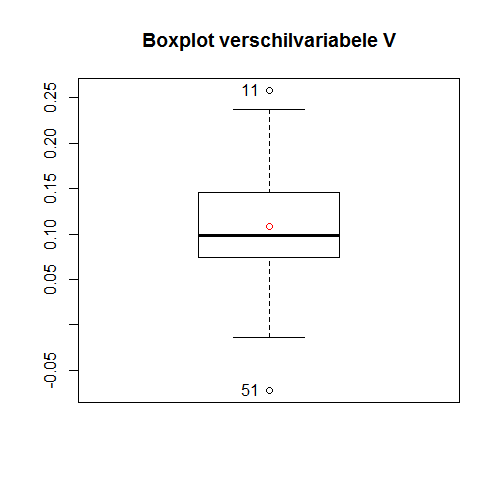
\includegraphics[scale=0.27]{data/Boxplot_verschilvariabele.png}
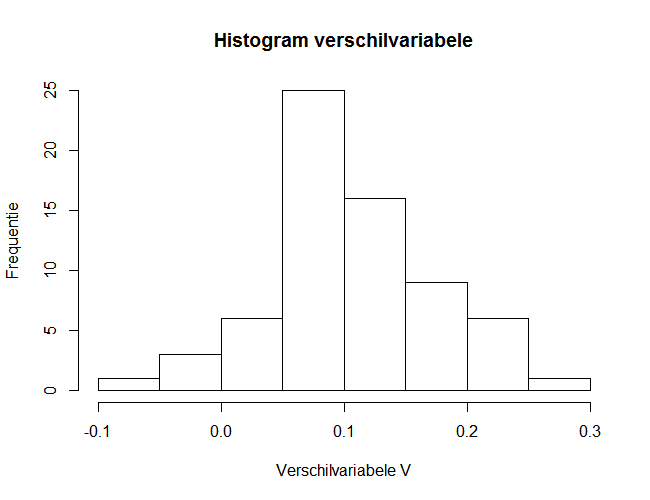
\includegraphics[scale=0.27]{data/histogram_verschilvariabele.png}
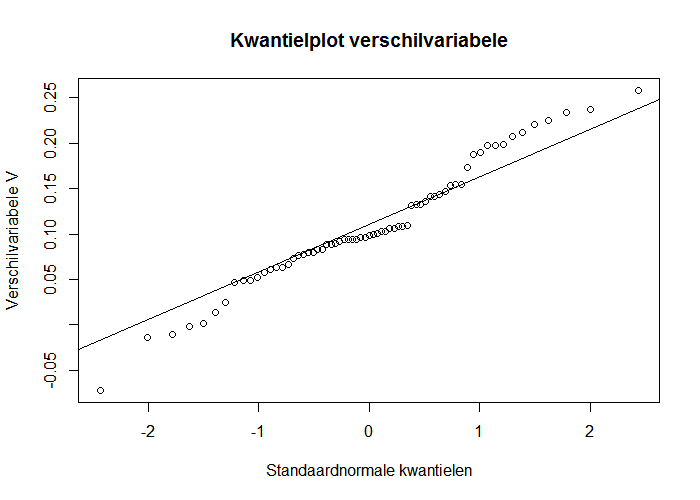
\includegraphics[scale=0.25]{data/kwantielplot_verschilvariabele.png}
\caption{Een boxplot, histogram en kwantielplot van de verschilvariabele V}
\label{fig:Graph}
\end{figure}

De boxplot laat zien dat er 2 waarnemingen buiten de snorharen liggen, dit zouden uitschieters kunnen zijn. Verder zijn de snorharen even lang en ligt het gemiddelde (rode cirkel) dicht bij de mediaan, dit wijst op een normale verdeling. Ook merken we op dat de mediaan iets lager ligt dan het midden, dit kan wijzen op een (licht) rechtsscheve verdeling. \\
\-\hspace{0.5cm}Het histogram laat een benaderende klok-curve zien, dit wijst op een normale verdeling. De rechterstaart is een beetje langer, dit kan opnieuw wijzen op een (licht) rechtsscheve verdeling.\\
\-\hspace{0.5cm}Vervolgens laat de kwantielplot benaderend een rechte zien, dit wijst opnieuw in de richting van een normale verdeling. Bij de kwantielplot merken we wederom twee afwijkende waarnemingen op die uitschieters zouden kunnen zijn.

\textbf{Formeel}\\
We gaan testen of de verdeling normaal is aan de hand van de Shapiro-Wilk test. We gebruiken de volgende hypothesen hiervoor:

\begin{center}
H${_0}$: De gegevens komen uit een normale verdeling. \\
H${_1}$: De gegevens komen niet uit een normale verdeling.
\end{center}

De test-waarde $w=0.97497$, {\it P-waarde} $= 0.1946$ en aangezien {\it P-waarde} $> \alpha$, kunnen we H$_{0}$ niet verwerpen en bevestigen we dat de verschilvariabele {\it V} normaal verdeeld is onder significantieniveau $\alpha = 0.05$.

We nemen verder aan dat waarneming 11 en 51 redelijk sterk verschillen van de andere waarnemingen, maar niet genoeg om te besluiten dat het uitschieters zijn.

\subsection{Uitvoering hypothesetesten}
Als eerste berekenen we de testwaarde aan de hand van de teststatistiek
\begin{center}
$T = \frac{\overline{V}}{S_{v}/\sqrt{n}} \rightarrow t = 13.391$ met $S\SPSB{2}{v}=\frac{1}{n-1} \sum\limits_{i=1}^n (V_{i} - \overline{V})^{2}$.
\end{center}
Deze testwaarde levert ons de P-waarde

\begin{center}
$P(T > t) = P(T > 13.391) = 2.2 \times 10^{-16} \approx 0$ met $T \sim t_{n-1} = t_{66}$. 
\end{center}

De P-waarde is veel kleiner dan $\alpha$. We kunnen H$_{0}$ dus verwerpen en dit bevestigt H$_{1}$ op significantieniveau $\alpha=0.05$.
Als we het 100(1-$\alpha$)\%-betrouwbaarheidsinterval maken voor $\mu_{v}=E(X)-E(Y)$ dan krijgen we:

\begin{center}
[ $\overline{v}-t_{n-1,\alpha/2}\frac{s_{v}}{\sqrt{n}}$ , $+\infty$ [\\
$\longrightarrow$
[ $0.0951823$, $+\infty$ [
\end{center}

Zoals verwacht na het berekenen van de P-waarde, is $0$ geen element van dit interval en kan men opnieuw H$_{0}$ verwerpen op significantieniveau $\alpha=0.05$.

\subsection{Besluit}
Aan de hand van P-waarde $2.2 \times 10^{-16}$ kunnen we H$_{0}$ verwerpen op significantieniveau $\alpha=0.05$. We kunnen besluiten dat $\mu_{v} > 0 $, met andere woorden is de gemiddelde BMI-waarde van vrouwen in het continent Afrika significant gestegen tussen 2007 en 2008.

\section{Opgave 2}
Een BMI-waarde is hoog als deze groter is dan de grenswaarde (die verschilt van land tot land), deze is laag als deze kleiner dan is of gelijk aan de grenswaarde is. Malaysia heeft een grenswaarde van {\it 23.1}. Is er een verschil in proportie ‘hoge BMI’ waarde bij mannen en vrouwen voor het land Malaysia (voor alle beschikbare jaren)?

\subsection{Hypothesetest}
We willen nagaan of er een verschil is tussen de proporties van hoge BMI-waarden bij mannen en vrouwen in Malaysia. Om dit te staven gebruiken we dus de tweezijdige test. De voorwaarde hiervoor is dat de gegevens onafhankelijk van elkaar zijn, dit wordt gecontroleerd in subsectie \ref{subsec:control2}. We gebruiken index 1 voor gegevens van de mannen en index 2 voor vrouwen. De hypothesen zijn dan als volgt:

\begin{center}
H${_0}$: $p_{1} = p_{2}$ \\
H${_1}$: $p_{1} \neq p_{2}$
\end{center}

\subsection{Controle voorwaarden}
\label{subsec:control2}
Om de voorwaarde van onafhankelijkheid na te gaan kunnen we volgende hypothesetesten gebruiken:

\begin{center}
H${_0}$: Het hoog of laag zijn van de BMI-waarde is onafhankelijk van het geslacht\\
H${_1}$: Het hoog of laag zijn van de BMI-waarde is afhankelijk van het geslacht
\end{center}

Bij volledige onafhankelijkheid kunnen we bepaalde waarden verwachten, zo is de

\begin{center}
$\textnormal{verwachte waarde} = \frac{\textnormal{rijtotaal } * \textnormal{ kolomtotaal}}{\textnormal{n}}$
\end{center}

Aan de hand hiervan bekomt men de tabel met de verwachte waarden.

\begin{table}[h!]
\begin{center}
 \begin{tabular}{c | c c | c} 
  & Hoog BMI & Laag BMI \\
 \hline
 Mannen & 17.5 & 11.5 & 29\\ 
 Vrouwen & 17.5 & 11.5 & 29\\
 \hline
  & 35 & 23 & 58\\
\end{tabular}
\end{center}
\caption{verwachte waarden bij onafhankelijkheid}
\label{table:1}
\end{table}

De geobserveerde waarden zijn zoals volgt.

\begin{table}[h!]
\begin{center}
 \begin{tabular}{c | c c | c} 
  & Hoog BMI & Laag BMI \\
 \hline
 Mannen & 14 & 15 & 29\\ 
 Vrouwen & 21 & 8 & 29\\
 \hline
  & 35 & 23 & 58\\
\end{tabular}
\end{center}
\caption{geobserveerde waarden}
\label{table:2}
\end{table}

Deze geobserveerde waarden verschillen van de verwachte waarden maar op het eerste zicht lijkt het verschil niet significant.

Om de onafhankelijkheid formeler aan te tonen berekenen we als eerste de testwaarde. De chi-kwadraat($X^{2}$)-teststatistiek is gedefinieerd als

\begin{center}
$X^{2} = \sum\limits_{i=1}^r \sum\limits_{j=1}^k \frac{(n_{ij}-nf_{i+}f_{+j})^{2}}{nf_{i+}f_{+j}}$ waarbij $X^{2} \approx _{H_{0}} \chi\SPSB{2}{v}$ met $v = (r-1)(k-1)$, \\
waarbij $n_{ij}$ de geobserveerde waarde is en $nf_{i+}f_{+j}$ de verwachte waarde.
\end{center}

Dit geeft ons de testwaarde $\chi^{2}=2.5938$. Hiermee berekenen we de P-waarde

\begin{center}
$P(X^{2}>\chi^{2}) = P(X^2 > 2.5938) = 0.1073$ met $X^2 \sim \chi\SPSB{2}{1}$.
\end{center}

De P-waarde is groter dan $\alpha$ en bijgevolg kunnen we H$_{0}$ niet verwerpen op significantieniveau $\alpha=0.05$. We nemen dus aan dat de gegevens onafhankelijk zijn van elkaar en dus is aan de voorwaarde voldaan.

\newpage

Bijkomende voorwaarden om de testwaarde te kunnen gebruiken, die gebruik maakt van een gewogen gemiddelde van $\hat{P_{1}}$ en $\hat{P_{2}}$ zijn:

\begin{center}
$n_{1}\hat{p_{1}} \geqslant 5$, $n_{1}(1-\hat{p_{1}}) \geqslant 5 \rightarrow 14 \geqslant 5, 15 \geqslant 5$\\
$n_{2}\hat{p_{2}} \geqslant 5$, $n_{2}(1-\hat{p_{2}}) \geqslant 5 \rightarrow 21 \geqslant 5, 8 \geqslant 5$\\
\end{center}

Deze voorwaarden zijn ook voldaan.

\subsection{Uitvoering hypothesetesten}
Als eerste berekenen we de testwaarde aan de hand van de teststatistiek

\begin{center}
$Z = \frac{\hat{P_{1}}-\hat{P_{2}}}{\sqrt{\hat{P_{0}}(1-\hat{P_{0}})\left(\frac{1}{n_{1}}+\frac{1}{n_{2}}\right)}} \rightarrow z = -1.878945$ met $Z \approx N(0,1)$.
\end{center}

Aan de hand van deze testwaarde bekomen we de P-waarde

\begin{center}
$2P(Z>|z|) = 2P(Z > 1.878945) = 0.06025$ 
\end{center}

De P-waarde is groter dan $\alpha$. We kunnen H$_{0}$ dus niet verwerpen op significantieniveau $\alpha = 0.05$.

Het 100(1-$\alpha$)\%-betrouwbaarheidsinterval wordt gegeven door

\begin{center}
[ $\hat{p_{1}}-\hat{p_{2}}-z_{\alpha/2}\sqrt{\frac{\hat{p_{1}}(1-\hat{p_{1}})}{n_{1}}+\frac{\hat{p_{2}}(1-\hat{p_{2}})}{n_{2}}}$, $\hat{p_{1}}-\hat{p_{2}}+z_{\alpha/2}\sqrt{\frac{\hat{p_{1}}(1-\hat{p_{1}})}{n_{1}}+\frac{\hat{p_{2}}(1-\hat{p_{2}})}{n_{2}}}$ ]\\
$\longrightarrow$
[ $-0.485383337$,  $0.002624717$ ]
\end{center}

Wederom zoals verwacht is 0 een element in dit interval en bijgevolg valt H$_{0}$ niet te verwerpen op significantieniveau $\alpha=0.05$.

\subsection{Besluit}
Aan de hand van de gevonden P-waarde van 0.06025 kunnen we de nulhypothese niet verwerpen en behouden we dus $p_{1} = p_{2}$, we kunnen dus besluiten dat er geen significant verschil is in de proporties tussen mannen en vrouwen omtrent hoge BMI-waarden, in Malaysia, gemeten van 1980 tot en met 2008.

\newpage
\section*{Bijlagen}
\lstinputlisting[float=ht,frame=tb,caption=R script,label=listing1]{script.tex}
\lstinputlisting[float=ht,frame=tb,caption=R output,label=listing2]{output.tex}

\end{document}
